\documentclass[11pt]{article}
\usepackage{amsfonts}
\usepackage{amsmath}
\usepackage{amsthm}
\usepackage{amssymb}
\usepackage{mathrsfs}
\usepackage[fit]{truncate}
\usepackage{acl2012}
\usepackage{times}
\usepackage{latexsym}
\usepackage{amsmath}
\usepackage{url}
\usepackage{graphicx}
\usepackage{caption}
\usepackage{multirow}
\usepackage{dblfloatfix}
\usepackage{float}
\usepackage{subfloat}
\usepackage{subcaption}

\setlength\titlebox{5cm}    % Expanding the titlebox

\newcommand{\affliationPenn}{\ensuremath{{}^\text{1}}}
\newcommand{\affliationJHU}{\ensuremath{{}^\text{2}}}

\title{The Language Demographics of  Amazon Mechanical Turk : Response  to Reviewers}

\author{Ellie Pavlick\affliationPenn \ \ \ \ \ Ann Irvine\affliationJHU  \ \ \ \ \ Dmitry Kachaev\affliationJHU  \ \ \ \ \  Chris Callison-Burch\affliationPenn$^{,}$\affliationJHU \\
\affliationPenn Computer and Information Science Department, University of Pennsylvania \\
\affliationJHU Human Language Technology Center of Excellence, Johns Hopkins University \\
  }
  
% Anonymized for submission
\author{}

\date{}

\begin{document}
\maketitle

\begin{figure}
\centering
\begin{subfigure}[b]{1\linewidth}
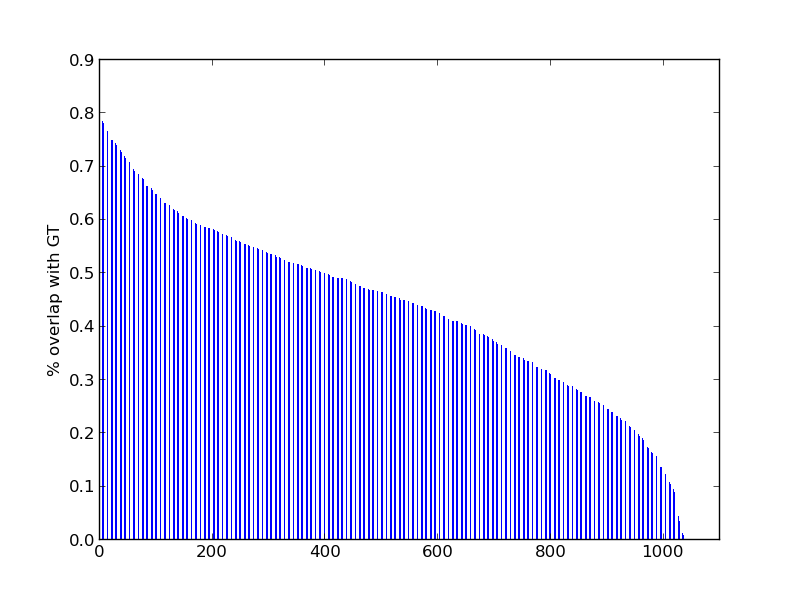
\includegraphics[width=\textwidth]{figures/turker-googmatch-distribution.png}
\caption{Individual turker overlap with google translate. We believe the inflection point at ~60\% overlap with Google suggests a reasonable cutoff by which to filter workers. Workers with \textgreater 60\% overlap can be reasonably considered to be cheating and can be removed.}                
\label{dist}
\end{subfigure}
\begin{subfigure}[b]{1\linewidth}
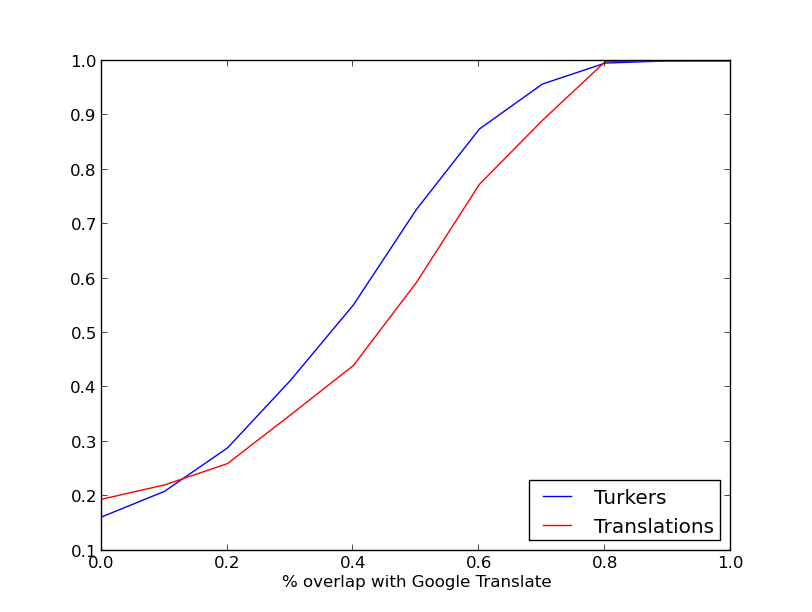
\includegraphics[width=\textwidth]{figures/google-cdf-googlangs.png}
\caption{Cumulative distribution of overlap with Google translate for workers and translations. We see that eliminating all workers with \textgreater 60\% overlap with google translate still preserves \textgreater 80\% of workers and \textgreater 70\% of translations.}
\label{cdf}
\end{subfigure}
\caption{}\label{cheaters}
\end{figure}

\section{Use of Google Translate}

The primary concern across reviewers was the high amount of overlap between workers' translations and translations available through online resources, i.e. Google Translate. The editor summarized : 
\begin{quote}
All reviewers had issues with the amount of cheating taking place among Turkers. It would be useful to quantify/detect this and remove such participants from your results.
\end{quote}

We took at closer look at the amount of overlap with Google translate in our collected translations in order to address this issue. We found that while overall overlap is high, it is not consistantly high across all turkers. Figure \ref{dist} shows that while a small number of turkers have a very high amount of overlap with Google (near 80\%) the majority overlap less than half of the time. 

As Reviewer E noted : 

\begin{quote}
..it is quite possible that a fluent speaker of a language provides the same translation as Google Translate for a given word.  In other words, the performance results are inconclusive.
\end{quote}

We see a clear inflection near the 60\% overlap point, suggesting that this cutoff may work well to eliminate turkers who are likely using Google Translate to cheat without punishing those who are producing honest translations that happen to overlap with Googe Translate.

Figure \ref{cdf} shows that removing workers with suspiciously high overlap with Google retains the majority of workers and translations, and will not greatly decrease the size of the study. 

We have rerun the quality analysis in the paper, omitting workers with \textgreater 60\% overlap with Google Translate. The quality scores and rankings do not change substantially. For reference, figure 2 from the paper is reproduced in figure \ref{qual}, both with and without the high-overlap Turkers included. 


\begin{figure}
\centering
\begin{subfigure}[b]{1\linewidth}
\includegraphics[width=\textwidth]{figures/fig2all_errorbars.png}
\caption{All turkers.}                
\label{dist}
\end{subfigure}
\begin{subfigure}[b]{1\linewidth}
\includegraphics[width=\textwidth]{figures/fig2filter_errorbars.png}
\caption{Turkers with \textless 60\% overlap with Google Translate.}
\label{cdf}
\end{subfigure}
\caption{Qualities for languages with \textgreater 50 turkers. Dark blue shows quality measured by perfect match on the control translation. Light blue indicates quality measured by included synonymous translations.}\label{qual}
\end{figure}


\section{Robustness of results to removing few big players}

The editor and reviewer G highlighted the possibility that the quality results are due to a few large players, and may not be robust if the experiment were rerun with a different group of workers : 
\begin{quote}
It is possible that a small number of workers could have driven response accuracies for some languages. The authors could have accounted for this in a straightforward way by regressing out the contributions of individual workers, e.g. by using random effects models.
\end{quote}
We ran a random effects model and found blah blah blah blah blah blah blah. 

\begin{figure}
\includegraphics[width=1\linewidth]{figures/turker_hit_contributions.png}
\caption{Contributions of individual turkers to the overall number of HITs in each language. The dark blue bar represents the proportion of total HITs which were completed by the 10 highest-contributing turkers. The next darkest bar represents the next 10 highest-contributing turkers, and likewise for the thrid and forth darkest. The final bar represents the remaining turkers which were not one of the top 40 contributors.}
\label{numhits}
\end{figure}


\section{Extrinsic evalutation of mturk data for SMT}

All the reviewers expressed desire for further evidence of the usefulness of the Turker-provided translations for statistical machine translation, and the possibility of extending the demonstrated methods to multiple word translations. The editor requests :

\begin{quote}
It would be interesting to show that the proposed approach brings an advantage over current SMT technology, i.e., improves lexical translations for an existing SMT system....It would also be interesting to assess whether your results carry over to multiple words and/or sentences. 
\end{quote}

Previous work by Matt Post in the 2010 WMT has demonstrated not only that turkers are able to provide high quality translations of complete sentences, but also that these translations, when added into an SMT pipeline, measurably improve translation quality. 

\begin{table}[t]
\centering
\begin{tabular}{l|rr}
  language  & SAMT &  Google \\
  \hline\hline
  Bengali    & 13.53  &  20.01 \\
  Hindi      & 17.29  & 25.21 \\  
  Malayalam    & 14.28  & - \\      
  Tamil      &  9.85  &  13.51 \\  
  Telugu     & 12.61  & 16.03  \\  
  Urdu        & 20.99  & 23.09 \\   
\end{tabular}
\caption{BLEU scores translating into English (four references).  BLEU
scores are the mean of three MERT runs.}
\label{table:bleu}
\end{table}

\begin{figure*}[t]
  \centering
  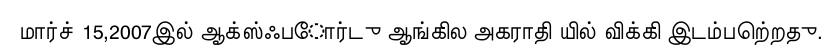
\includegraphics[width=\textwidth]{figures/tamil.png}
  \begin{tabular}{l}
    \hline
    In March 15,2007 Wiki got a place in Oxford English dictionary. \\
    On March 15, 2007 wiki was included in the Oxford English
    dictionary. (5) \\
    ON MARCH 15, 2007, WIKI FOUND A PLACE IN THE OXFORD ENGLISH
    DICTIONARY \\
    March 15, 2007 oxford english index of wiki's place. \\ \\

  \end{tabular}
  \caption{An example of the variance in translation quality for the
    human translations of a Tamil sentence; the formatting of the
    translations has been preserved exactly.  The parenthesized number
    indicates the number of votes received in the voting task
    (\S\ref{section:votes}).}
  \label{figure:variance}
\end{figure*}

\section{Affect of time of day when HIT was posted}

Reviewer F raised an interesting question about the affect of time of day on Turker activity : 

\begin{quote}
Did the authors take into account time of day, when the HIT was posted etc. to get a sense of whether one time of day is more optimal than others for each language? Does it matter at all?
\end{quote}
Figure \ref{time} shows the activity over a 24 hour day for 23 languages with greater than 100 turkers each. The plot shows that activity does vary across time zones, and suggests that choosing the release time intelligently based on the HIT language is likely to affect how quickly it is completed.
\begin{figure*}
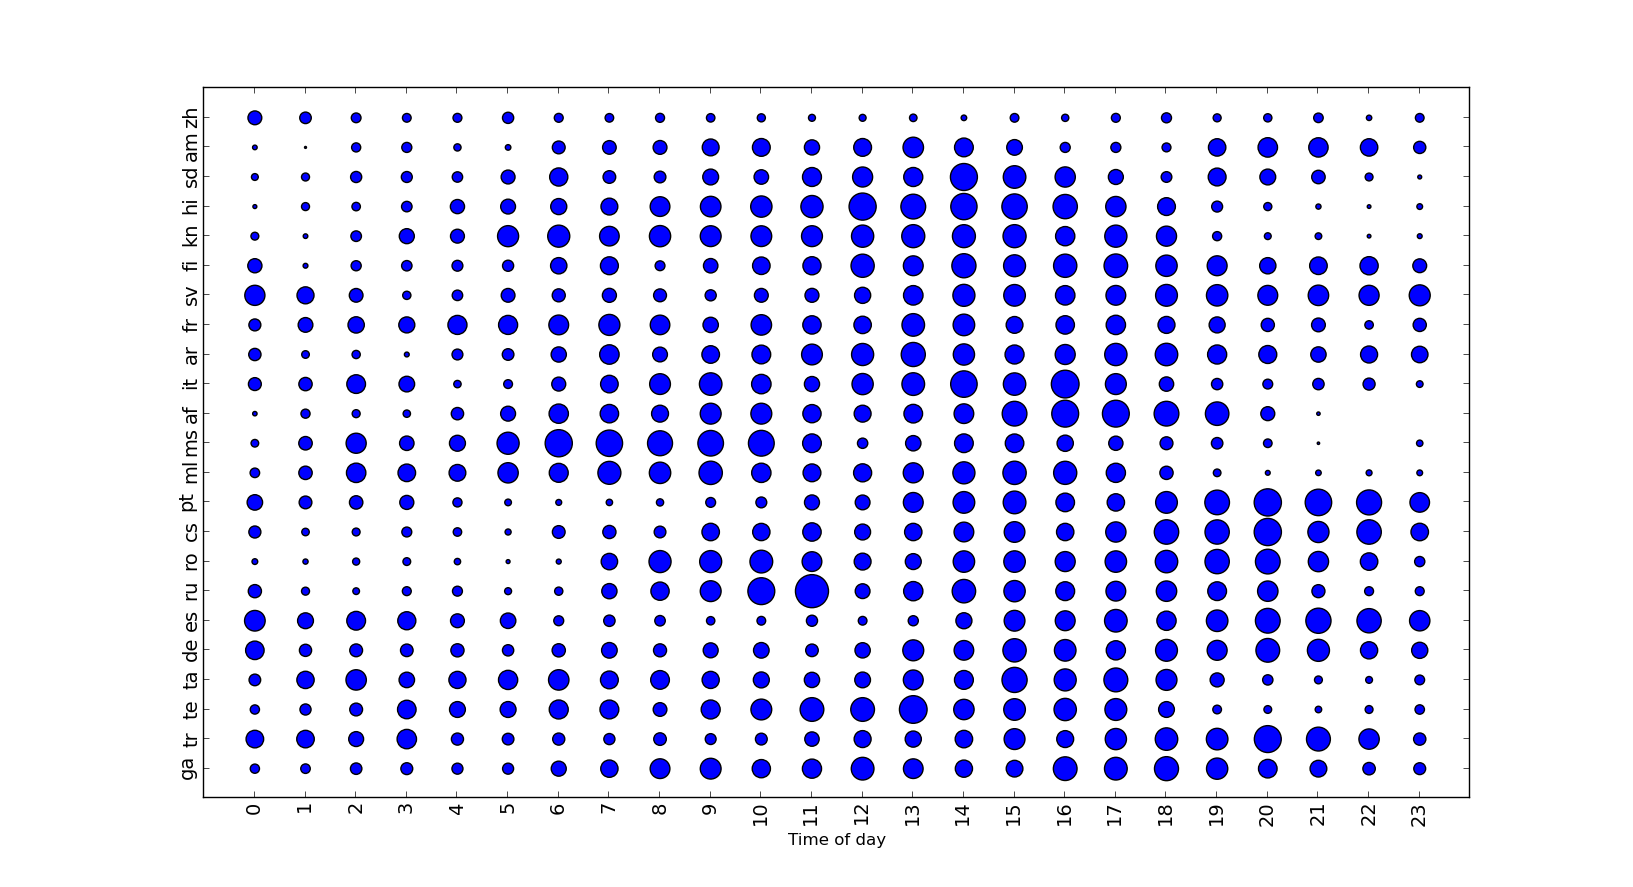
\includegraphics[width=1\linewidth]{figures/times.png}
\caption{Number of HITs completed during each hour of the day for languages with \textgreater 100 turkers.}
\label{time}
\end{figure*}

\section{Changes in results if study continued over time}

Reviewer B asked : 
\begin{quote}
The authors ran an experiment over 3.5 months, but I wonder how the demographics change over time. Are there seasonal effects in the workforce? Has it changed over the past year? And more importantly, will it change substantially in the future? I'm somewhat skeptical that these demographics will remain constant, especially as Amazon rolls out changes to the service.
\end{quote}

While we agree that the questions posed are very interesting, we feel that answering these questions is the subject of another study. Our study is aimed at capturing the current demographics of Mechanical Turk, and proposing a way to empiracally validate self-reported demographic information about language skills. It is true that the current demongraphic makeup of MTurk workers is likely to shift, but the time and expense of tracking these changes over time puts the reviewer's questions outside the scope of this project.

\section{Accuracy of Geolocation}

We understand that geolocation is not perfect, which is why we propose the use of location data as just one of several criteria by which to identify likely qualified translators. The trends that we observe in our analysis, where we show that turkers geolocated within a region likely to speak the source language being translated tend to perform better on our controls, coincide with what we would expect to see if geolcation were accurate. This seems to support the assumption that, on average, the geolocation is performing sufficiently well.

\end{document}
